%----------------------------------------------------------------------------------------
%
% LaTeX-mall för examensarbeten vid LNU
% Skapad av Marcus Wilhelmsson, Institutionen för Datavetenskap
% Fakulteten för Teknik
% Linnéuniversitetet
%
% Licens: Creative Commons
%
%----------------------------------------------------------------------------------------

%----------------------------------------------------------------------------------------
%	Inställningar och dokumentkonfiguration
%----------------------------------------------------------------------------------------
\documentclass[a4paper,12pt]{article} % A4-sida och 12 punkters fontstorlek

\usepackage[T1]{fontenc} % 8-bitarskodning som har 256 glyfer
\usepackage{times} % Typsnitt i dokumentet
\usepackage[swedish,english]{babel} % Svenskt språk, engelska för extra abstract
\usepackage[utf8]{inputenc} % För svenska tecken (UTF-8)
\usepackage{dtklogos} % Logos för t.ex. LaTeX, BibTeX, etc.
\usepackage{wallpaper} % Bakgrundsbild
\usepackage[absolute]{textpos} % Möjlighet att absolutpositionera text
\usepackage[top=2cm, bottom=2.5cm, left=3cm, right=3cm]{geometry} % Ställ in marginaler
\usepackage{appendix} % Stöd för separat hantering av bilagor
\usepackage[parfill]{parskip} % Tar bort indentering vid ny rad
\usepackage{csquotes} % Används för att hantera citat
\usepackage{float} % Används för att placera figurer och tabeller rätt.

% Används för att texten ska hamna ovanför tabeller och för bra mellanrum.
\floatstyle{plaintop}
\restylefloat{table}
\usepackage[tableposition=bottom]{caption}

\setcounter{secnumdepth}{3} % Fem nivåer av underrubriksnumrering
\setcounter{tocdepth}{3} % Fem nivåer av underrubriksnumrering i innehållsförteckning

\usepackage{sectsty} % Ändra storlek på section och subsection till 12 punkter
\sectionfont{\fontsize{14}{15}\selectfont}
\subsectionfont{\fontsize{12}{15}\selectfont}
\subsubsectionfont{\fontsize{12}{15}\selectfont}

%----------------------------------------------------------------------------------------
%	Denna del används för att skapa boxen med författare, handledare, etc.
%----------------------------------------------------------------------------------------
\newsavebox{\mybox}
\newlength{\mydepth}
\newlength{\myheight}

\newenvironment{sidebar}%
{\begin{lrbox}{\mybox}\begin{minipage}{\textwidth}}%
{\end{minipage}\end{lrbox}%
 \settodepth{\mydepth}{\usebox{\mybox}}%
 \settoheight{\myheight}{\usebox{\mybox}}%
 \addtolength{\myheight}{\mydepth}%
 \noindent\makebox[0pt]{\hspace{-20pt}\rule[-\mydepth]{1pt}{\myheight}}%
 \usebox{\mybox}}

%----------------------------------------------------------------------------------------
%	Titel-sektion
%----------------------------------------------------------------------------------------
\newcommand\BackgroundPic{
    \put(-2,-3){
    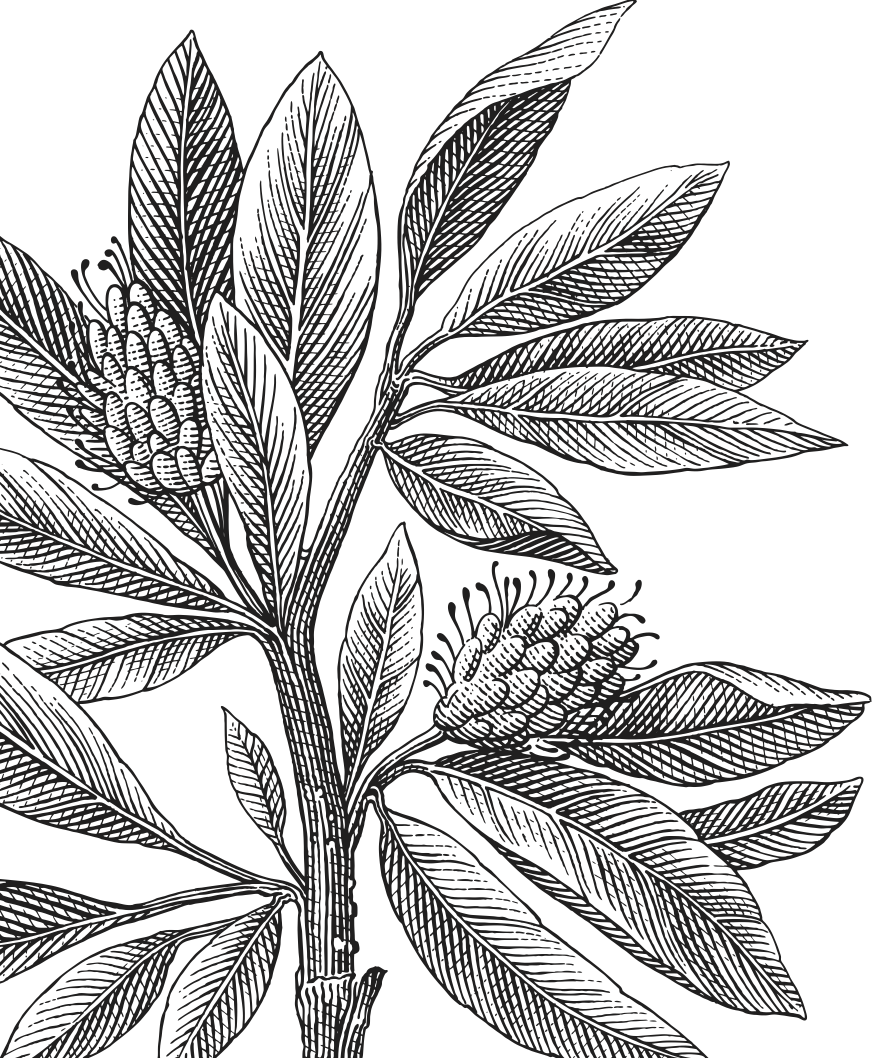
\includegraphics[keepaspectratio,scale=0.3]{img/lnu_etch.png} % Bakgrundsbild
    }
}
\newcommand\BackgroundPicLogo{
    \put(30,740){
    
\includegraphics[keepaspectratio,scale=0.10]{img/logo.png} % Logga i övre vänstra hörnet
    }
}

\title{
\vspace{-8cm}
\begin{sidebar}
    \vspace{10cm}
    \normalfont \normalsize
    \huge Dokumenttyp\\ % Dokumentets typ, t.ex. Examensarbete
    \vspace{-1.3cm}
\end{sidebar}
\vspace{3cm}
\begin{flushleft}
    \huge Rubrik\\ % Dokumentets rubrik
    \it \large Examensarbete under arbete % Dokumentets underrubrik
\end{flushleft}
\null
\vfill
\begin{textblock}{6}(10,13)
\begin{flushright}
\begin{minipage}{\textwidth}
\begin{flushleft} \large
\emph{Författare:} John \textsc{Smith}\\ % Författare
\emph{Handledare:} Dr.~Foo \textsc{Bar}\\ % Handledare
\emph{Examinator:} Dr.~Mark \textsc{Brown}\\ % Examinator
\emph{Termin:} HT2013\\ % Termin
\emph{Ämne:} Någonvetenskap\\ % Ämne
\emph{Nivå:} G2F\\ % Nivå
\emph{Kurskod:} 2DVXXX % Kurskod
\end{flushleft}
\end{minipage}
\end{flushright}
\end{textblock}
}

\date{} % Dagens datum, tomt i detta fallet. Använd \today för dagens datum.

\begin{document}
\renewcommand{\figurename}{Figur} % Byt ut "Figure" mot "Figur".
\renewcommand{\tablename}{Tabell} % Byt ut "Table" mot "Tabell".
\pagenumbering{gobble}
\newgeometry{left=5cm}
\AddToShipoutPicture*{\BackgroundPic} % Lägger in backgrundsbild på första sidan
\AddToShipoutPicture*{\BackgroundPicLogo} % Lägger in LNU-logga på första sidan
\maketitle % Skriv ut titeln
\restoregeometry
\clearpage

%----------------------------------------------------------------------------------------
%	Svensk och engelsk version av abstract
%----------------------------------------------------------------------------------------
\pagenumbering{roman}
\selectlanguage{swedish}
\begin{abstract}
\noindent Uppsatsen kan ha en sammanfattning eller ett abstrakt. Det är en viss skillnad på dessa. Om uppsatsen skrivs på svenska har man ofta både en svensk och en engelsk sammanfattning. Sammanfattningen eller abstraktet skrivs alltid sist när allt annat är färdigskrivet. Tempusformen är imperfekt, dåtid, det vill säga vad som har gjorts.\\

\noindent En sammanfattning är en kortfattad återgivelse av uppsatsens hela innehåll. Sammanfattningen bör vara max 1 sida lång oavsett hur lång uppsatsen är. Ett bra sätt att skriva en bra sammanfattning kan vara att skriva en eller ett par meningar om varje kapitel i uppsatsen, det vill säga inledning, syfte, teori, metod, resultat, analys, diskussion och slutsats. Sammanfattningen kan gärna delas upp i styckeindelningar för att öka läsbarheten.\\

\noindent Ett abstrakt är ett mer vetenskapligt sätt att sammanfatta uppsatsen. Abstraktet bör inte vara längre än ett stycke och är aldrig uppdelat i mer än ett stycke. I abstraktet skall man besvara frågorna:
\begin {itemize}
\item Vad var problemet?
\item Vad har man gjort för att belysa problemet?
\item Vad har man kommit fram till?
\end {itemize}

\noindent Ibland följs abstraktet av några nyckelord, som är representativa för uppsatsens område.\\

\noindent Utifrån att ha läst sammanfattningen eller abstraktet skall man tydligt förstå vad uppsatsen handlar om. Man brukar säga att titeln på uppsatsen sedan är en sammanfattning av sammanfattningen. Det vill säga att titeln på uppsatsen också skall ge en tydlig indikation på vad uppsatsen handlar om. Om man har nyckelord är det en god idé att titeln innehåller en stor del av dessa. Då vet man att man har en rättvisande titel. I våra datavetenskapliga rapporter använder vi oss av upplägget för abstrakt.\\

\noindent\textbf{Nyckelord:}
\end{abstract}
\selectlanguage{english}
\begin{abstract}
\noindent A translation will come.\\

\noindent\textbf{Keywords:}
\end{abstract}
\selectlanguage{swedish}

\newpage

%----------------------------------------------------------------------------------------
%	Svensk och engelsk version av förord
%----------------------------------------------------------------------------------------
\textbf{\large{Förord}}\\

Man kan ha ett förord i uppsatsen om man vill, men det behövs inte. I detta kan man få skriva mer personliga reflektioner kring uppsatsskrivandet. Det kan exempelvis vara varför man själv personligen tyckte att det var ett intressant ämne att skriva om eller om man upplevt det som särskilt svårt eller givande att skriva uppsatsen.

Det är också i förordet man kan passa på att tacka personer som varit till särskild hjälp under uppsatsskrivandet, exempelvis om man haft någon kontaktperson på ett företag som hjälpt till, de som har deltagit i intervjuer eller enkäter, om man fått någon finansiering från någon eller om man haft någon som hjälpt till med att korrekturläsa.

Förordet bör inte bli långrandigt, max en halv sida. Tänk också på anonymitet och sekretess innan du nämner personer vid namn. Man kan tacka personer ändå, utan att skriva deras namn.

\newpage

%----------------------------------------------------------------------------------------
%	Innehållsföreteckning
%----------------------------------------------------------------------------------------
\pagenumbering{gobble} % Stäng av sidnumrering för innehållsförteckningssidan
\tableofcontents % Innehållsförteckning

\newpage % Ny sida
\pagenumbering{arabic} % Påbörja sidnumrering på 1

%----------------------------------------------------------------------------------------
%	Rubrik 1
%----------------------------------------------------------------------------------------
\section{Rubrik 1}
Enligt \cite{small} är detta en rubrik. Enligt \cite{big} är även detta en rubrik.

%----------------------------------------------------------------------------------------
%	Underrubrik 2
%----------------------------------------------------------------------------------------
\subsection{Underrubrik 2}
Lorem ipsum dolor sit amet, consectetur adipiscing elit. Pellentesque convallis arcu elit, sit amet dictum nibh semper id. Quisque non iaculis est. Mauris ornare auctor scelerisque.

%----------------------------------------------------------------------------------------
%	Under-underrubrik 3
%----------------------------------------------------------------------------------------
\subsubsection{Underrubriksnivå 3}
Nunc molestie libero in quam commodo, id volutpat justo vehicula. Aliquam tristique leo et ullamcorper dapibus. Sed eu blandit lorem. Phasellus fermentum risus ac risus porttitor consectetur. Nunc euismod ultricies pellentesque. Quisque id dolor lorem. Nulla sollicitudin dignissim quam, a blandit sapien lobortis et.

\section{Introduktion}
% \emph innebär emphasize, d.v.s. betona eller framhåll -> kursiv stil
\emph{Inled med lite text som beskriver innehållet i kapitlet.}\\
Detta kapitel skall beskriva vad uppsatsarbetet kommer att handla om och kan delas upp i olika underrubriker. Nedan finns ett förslag, men vilka man använder beror lite på vilken typ av uppsats man skriver och vilken typ av undersökning man gör. Det är också möjligt att ha rubrikerna i en annan ordning om man så önskar.

Introduktionen skall väcka läsarens intresse för uppsatsen och återge tillräckligt mycket bakgrundsfakta för att läsaren skall kunna förstå problemformuleringen. Introduktionen bör inte bli för lång, då är det lätt att man redan här tappar läsarens intresse. Därför skall den enbart innehålla sådana beskrivningar som är relevanta.
Introduktionen skrivs med en blandning av presens, imperfekt och futurum. Exempelvis presens för vad man själv och andra tycker och hur olika saker förhåller sig och sådant som gäller just nu i skrivandets stund. Imperfekt för vad andra forskare har gjort och kommit fram till. Futurum för vad man i sin undersökning avser att göra och vad man i uppsatsen kommer att beskriva.
Man kan skriva en första version av introduktionen som första steg i uppsatsarbetet. Under arbetets gång får man kanske ändra lite på den. När uppsatsen börjar bli klar går man sedan tillbaka och justerar introduktionen slutligt. Det händer att syfte och frågeställningar ändras under arbetets gång. Det kan också tillkomma ny tidigare forskning. Slutligen vill man också gärna finslipa lite till på sin inledning när man har resultatet, diskussionen och slutsatsen klar, så att dessa blir samstämmiga.

% lägg in en underrubrik (\subsection -> spillutrymme)
\subsection{Inledning/Bakgrund}
Beskriv mycket kort och i allmänna ordalag vad uppsatsen kommer att handla om. Beskriv kanske hur du kom på att skriva om detta. Att man glider in på ett visst område kan bero på att man inledningsvis har en undran. Denna undran är inte så precis som en forskningsfråga, men kommer kanske att leda fram till en sådan. Man bör också motivera varför det ämne man valt är intressant och relevant. Ett bra sätt kan vara att ta upp något från media eller den allmänna samhällsdebatten för att visa att ämnet är aktuellt.

En del studier berör någon form av praktisk problemlösning, kanske på uppdrag av något företag. Beskriv då det praktiska problemområdet här. Det kan innebära en kort beskrivning av verksamheten och uppdraget.

I detta och kommande avsnitt kan man lämpligen använda sig av en så kallad ”tratteknik” när man skriver. Det innebär att man beskriver området väldigt brett till att börja med, för att sedan smalna av sig mer och mer tills man kommer ner till uppsatsens frågeställning.

\subsection{Tidigare forskning}
Här beskriver man kortfattat vad andra har gjort inom det område som uppsatsen skall beröra eller hur andra har försökt belysa eller lösa det problem som man avser att studera. Detta avsnitt skall bara innehålla korta och relevanta referat. Den litteratur man främst baserar sig på är uppsatser, vetenskapliga artiklar och böcker. Hänvisning till de referenser som man har använt skall göras löpande. Se i teorikapitlet i detta dokument hur dessa referenser skall göras.

Avsnittet kan också innehålla beskrivning av sådan teoretisk bakgrund som behövs för att beskriva problemet. Då gör man oftast en sammanfattning här och utvecklar sedan beskrivningarna mer i teorikapitlet.

\subsection{Problemformulering}
Här beskriver man det problem som man i uppsatsen avser att undersöka. För att arbetet skall räknas som en uppsats skall detta vara ett vetenskapligt problem. Inom den forskning som bedrivs inom datavetenskap finns dock möjligheten att också arbeta med ett praktiskt problem, men detta skall ändå vara kopplat till ett vetenskapligt problem. I så fall beskriver man här först det praktiska problemet och sedan det vetenskapliga problemet. Man kan tänka sig problemet som en slags kunskapslucka som man vill göra ett kunskapsbidrag till. Exempel på problem kan vara att man inte vet vad människor tycker i en viss fråga, att man inte vet hur något fungerar, att man inte vet vad ett visst problem beror på eller att det saknas metoder.

\subsection{Syfte och frågeställning/hypotes}
Syfte beskriver vad man avser att göra för att undersöka problemet och fylla kunskapsluckan. Man kan säga att det är en slags sammanfattning av genomförandet. Syftet bör även innehålla en precisering av vilken typ av kunskap man avser att producera. Exempelvis beskrivande kunskap, förklarande kunskap och normativ kunskap (vilket innebär metoder).

Beroende på om man arbetar deduktivt eller induktivt bör man sedan precisera sitt syfte i en eller flera hypoteser eller frågeställningar. En hypotes är ett antagande om hur något förhåller sig, som man avser att undersöka om det stämmer eller inte. Exempelvis att man utgår från att alla systemutvecklingsföretag följer en systemutvecklingsmetod, som man avser att undersöka om det stämmer eller inte. Hypotesen grundar sig alltid i teori eller tidigare forskning. Man måste alltså veta något innan man kan formulera en hypotes. Detta innebär att arbeta deduktivt.

Om man inte vet något (inte du personligen utan vetenskapssamhället) så får man istället arbeta induktivt. Då formulerar man en eller flera forskningsfrågor. Dessa frågor skall man besvara genom den undersökning man gör. Uppsatsens slutsats är därmed ett direkt svar på forskningsfrågorna. En forskningsfråga kan exempelvis vara vilka systemutvecklingsmetoder som används av systemutvecklingsföretag. Forskningsfrågorna är en tydligare precisering av den inledande undran som man kanske hade.

\subsection{Avgränsning/Begränsning}
Detta avsnitt är inte obligatoriskt att ha i en uppsats. Här tar man upp vad man inte avser att göra i sin undersökning. Det är viktigt att inte blanda ihop detta med det urval man beskriver i metodkapitlet. Man skall alltså inte här beskriva att man kommer att intervjua X och Y, men inte Z. Det är också avgränsning som är relevant för syftet i fråga. Man skall alltså inte precisera att man valt bort att studera resten av världen. En del avgränsningar känner man kanske till från början, medan andra naturligen tillkommer under arbetets gång. Motivera också varför detta inte kommer att studeras. Tid är ett vanligt motiv till varför aspekter måste väljas bort. Tänk dock på att beskriva det på ett professionellt sätt och man skall inte ursäkta sig.

\subsection{ Målgrupp}
Detta avsnitt är inte obligatoriskt. Däremot kan det vara bra både när man skriver och sedan för läsaren. Här beskriver man alltså vilka man avser att ge sitt kunskapsbidrag till och vilka man skriver uppsatsen för. Om jag som läsare står omnämnd i målgruppen, så vet jag ju att denna uppsats borde vara av intresse för mig att läsa.

Om man planerar att göra ett praktiskt bidrag till någon specifik grupp av personer eller verksamhet beskriver man det här. För att det skall vara en vetenskaplig uppsats räcker det dock inte med denna målgrupp. Det måste finnas en mer generell och vetenskaplig målgrupp. Att beskriva denna målgrupp här och hela tiden tänka på att man skriver för dem är därför ett bra sätt att se till att det blir en vetenskapligt godkänd uppsats.

Det räcker ju inte heller att ha handledaren och examinatorn som målgrupp. Om man inte kan komma på en bredare målgrupp har man kanske valt ett dåligt uppsatsämne som inte är så intressant, relevant och nyskapande.

\subsection{Disposition}
Detta avsnitt är inte obligatoriskt, men det kan vara bra att ha en beskrivning av vilka olika kapitel och avsnitt som uppsatsen innehåller och hur dessa förhåller sig till varandra. Man kan här också ge läsanvisningar för särskilda målgrupper av läsare om man så önskar.

\newpage

\section{Bakgrund/Teori}
\emph{Inled med lite text som beskriver innehållet i kapitlet.}\\
Här beskrivs uppsatsens bakgrund och eller teori. Kapitlet eller kapitlen delas in i valfria relevanta avsnitt. Det är möjligt att ha både ett bakgrundskapitel och ett teorikapitel om man tycker att detta behövs. Teorikapitlet kan komma som nummer 2, men det är också möjligt att lägga metodkapitlet före teorikapitel. Det beror på om man tycker att läsaren behöver känna till teorierna för att förstå tillvägagångssättet för undersökningen.

\subsection{Inledning}
Teorier beskriver och förklarar hur omvärlden och olika fenomen i den förhåller sig. Teorin används för att analysera, det vill säga beskriva och förklara det man studerar eller som utgångspunkt för att formulera en hypotes. Teorier beskrivs oftast i böcker, men kan även beskrivas i vetenskapliga artiklar.
Teorierna skall sammanfattas och återges kortfattat med referenser till litteraturen. Beskriv teorierna med egna ord. Citat kan användas, men bör göras sparsamt. Kanske inte hela teorin kommer att användas, beskriv då bara den del av teorin som används. Endast relevanta, det vill säga de teorier som man verkligen kommer att använda, ska beskrivas. Man bör dock visa på att man gjort ett medvetet val av teorier. Därmed kan man skriva några korta meningar om att dessa teorier finns, men dessa teorier har valts därför att… och så vidare. Man skriver ofta mycket i detta kapitel till att börja med som man sedan får ta bort. Se till att verkligen ”Kill your darlings”, dvs tänk efter om det verkligen passar in! Man skall också beskriva hur man kommer att använda teorierna i sin analys. Om man inte kan beskriva detta är det nog troligt att teorin inte heller är användbar och därmed bör tas bort. Om man beskriver flera teorier skall man också göra en tydlig koppling mellan teorierna.
I bakgrunden kan man utveckla beskrivningar av tidigare forskning, som inte fick plats i introduktionen. Om man gör en praktisk studie kan man också i detta kapitel göra en mer utförlig beskrivning av de praktiska förutsättningarna. Man kan också i ett bakgrundskapitel beskriva sådan teori som behövs för att beskriva problemet, men som inte kommer att användas i analysen. Exempel på detta kan vara definitioner av olika begrepp inom området.

\subsection{Löpande referenser}
Alla påståenden som man gör i detta kapitel måste kunna styrkas med referenser till litteratur. Detta gör man med så kallade löpande referenser eller källhänvisningar. All refererad litteratur skall också återfinnas i referenslistan i slutet av uppsatsen.

Löpande referenser kan göras på i huvudsak två olika sätt, se exempel 1 och 2. Det kan vara trevligt att växla lite mellan de två olika sätten, beroende på vad som passar. Man skall alltid använda författaren efternamn och publiceringsår. Detta räcker för att man skall kunna hitta referensen i referenslistan.\\

{\em Exempel 1:}\\
Mening mening mening mening \cite{sven01}.

Det finns många fina blommor \cite{sven01}.

{\em Exempel 2:}\\
Enligt Efternamn [\#] mening mening mening…

Enligt Svensson \cite{sven01} finns det många fina blommor.\\

Ibland finns det två författare till ett verk, då skriver man som i exempel 3. Om det finns tre eller fler författare skriver man som i exempel 4. Ibland vill man stärka ett påstående med två eller fler referenser, då gör man som i exempel 5. Referenserna ordnas då i bokstavsordning. \\

{\em Exempel 3:}\\
Enligt Efternamn1 och Efternamn2 [\#] mening mening mening mening.

Enligt Svensson och Öberg finns många fina blommor \cite{sven02}.\\

{\em Exempel 4:}\\
Enligt efternamn et al, \cite{Creswell2014} mening mening mening mening.

Enligt Svensson et al, \cite{sven07} finns det många fina blommor.\\

{\em Exempel 5:}\\
Mening mening mening mening [\#], [\#].

Det finns många fina blommor \cite{sven01}, \cite{sven02}.\\

Figurer och tabeller skall också ha en referens i dessa anges också oftast sidnummer. Även när man gör citat skall man ange sidnummer. Exempel 6 visar hur man skriver kortare citat och exempel 7 visar hur man skriver längre citat.\\

{\em Exempel 6:}\\
Text text. ”Citat citat citat…”  [\#, s. sidnummer]. Text text text text text och så vidare.

\begin{quotation}
Det finns manga finfina blommor \cite[s. 23]{Creswell2014} \\
\end{quotation}

{\em Exempel 7:}
\hyphenblockcquote{swedish}[s. 1]{Creswell2014}{
Text text text text text och så vidare. Citat citat citat citat citat. Citat citat citat citat citat citat. Citat citat citat citat citat citat. Citat citat citat citat citat citat. Text text text text text och så vidare. Citat citat citat citat citat. Citat citat citat citat citat citat. Citat citat citat citat citat citat. Citat citat citat citat citat citat.}
Text text text text text och så vidare. \\

Detta var de vanligaste fallen av hur man skriver löpande referenser. Det finns också ett antal mer speciella fall, exempelvis rapporter utgivna av myndigheter och webbsidor. Se därför också i metodlitteraturen kring hur man gör löpande referenser.

\subsection{Figurtexter}
Alla figurer och tabeller skall vara numrerade och ha en rubrik/förklarande text samt eventuell referens. Figurer är alla typer av modeller, bilder och även grafer och diagram. Numreringen ska göras för varje kapitel och då får första figuren i kapitel 2 nummer 2.1, nästa figur får nummer 2.2, första bilden i kapitel 3 får nummer 3.1 och så vidare. Tabeller har separat numrering, d v s rapportens första och andra tabell i kapitel två får då nummer 2.1 och 2.2.

\begin{figure}[H]
\begin{center}

\includegraphics[scale=0.5]{img/cirkvad}
\end{center}
\caption{Kvadrat och cirkel, [8].}
\label{cir_kvad}
\end{figure}

Figurer har figurtexten under figuren, se figur 2.1, medan tabeller har texten ovanför, se tabell 2.1. Alla figurer, tabeller och diagram skall också hänvisas till från den löpande texten och figuren eller tabellen skall placeras i så nära anslutning som möjligt till denna hänvisning. Figurer får läggas in mellan stycken, men texten får då enbart vara i linje med figuren och inte flöda tätt med figuren (det vill säga det får inte vara någon text till höger eller vänster om figuren). \\

\begin{table}[H]
\centering
\begin{tabular}{|r|r|r|}\hline
346 & 5 & 987 \\ \hline
989 & 2078 & 654 \\ \hline
45 & 765 & 2345 \\ \hline
\end{tabular}
\caption{En tabell med siffror.}
\label{tabell1}
\end{table}

\newpage

\section{Metod}
\emph{Inled med lite text som beskriver innehållet i kapitlet.}\\
I metodkapitlet beskriver man sitt vetenskapliga tillvägagångssätt. Det vill säga hur man har genomfört sitt arbete och hur man har kommit fram till sina resultat samt vilka metoder man har valt för att validera resultaten. Ett metodkapitel kan delas in i olika avsnitt. Nedan ges ett förslag till indelning. Metodkapitlet kan också läggas som kapitel 2, före teorikapitlet.

I en forskningsplan beskriver man kanske hur man planerar att gå tillväga i sitt arbete, alltså i tempusformen futurum. Metodkapitlet skall däremot vara skriver i imperfekt. Man kan skriva en version av metodkapitlet före genomförandet och sedan uppdaterar man och ändrar denna efter genomförandet. Var dock noga med att denna uppdatering verkligen görs!

I metodkapitlet är det viktigt att lägga fokus på den eller de metoder man har använt sig av. Man skall dock visa att man gjort ett medvetet och relevant val av metod. Man kan därför mycket kort nämna vilka metoder som finns som alternativ. Det skall finnas en tydlig motivering till det val av metod som man har gjort.

Metoder och tekniker beskrivs i litteratur. Det viktigaste är att i metodkapitlet beskriva hur man själv har gjort och sedan tar man stöd i litteraturen för att motivera detta. Man kan alltså mycket kort återge vad som står i litteraturen, men det är viktigt att metodkapitlet inte skall bli en metodlärobok.

\subsection{Vetenskaplig ansats}
I detta avsnitt kan man inledningsvis beskriva om man valt en induktiv eller deduktiv ansats. Man kan också beskriva om man kommer att göra en kvalitativ eller kvantitativ undersökning. Naturligtvis skall alla val motiveras.

\subsection{Datainsamling}
Här beskriver man vilka datainsamlingstekniker som man har använt sig av. Man bör kortfattat ta upp alternativ och diskutera varför dessa tekniker inte har valts. De vanligaste datainsamlingsteknikerna är:
\begin{itemize}
\item Enkäter
\item Intervjuer
\item Dokumentstudier
\item Observationer
\end{itemize}

\subsubsection{Urval}
När man samlar in data har man sällan möjlighet att göra det från alla inom det studerade området (populationen), vilket kallas att göra en totalundersökning. Oftast behöver man göra någon form av urval. Personer som tillfrågas i intervjuer och som observeras kallas informanter och personer som svarar på enkäter kallas respondenter. Det finns olika typer av urval som kan göras, exempelvis bekvämlighetsurval, strategiskt urval, kvoturval, representativt urval. Se i metodlitteraturen för närmare beskrivningar av dessa. I detta avsnitt beskriver man det urval som man har tillämpat och varför.

\subsubsection {Genomförande}
I detta avsnitt beskriver man genomförandet av datainsamlingen. Man beskriver exempelvis hur man gått tillväga för att utforma frågor till intervjuer eller enkäter. Själva intervjufrågorna och enkätformulären kan man gärna lägga i en bilaga, som man hänvisar till härifrån. Man beskriver hur intervjuer gjorts eller när enkäter skickats ut och hur, hur intervjuer dokumenterats och hur enkäter samlats in. Oftast får man inte svar på alla enkäter som man skickat ut. Här kan man också ange och diskutera den svarsfrekvens man haft. Det är viktigt att vara tydlig med hur man gått tillväga, men inte gå till överdrift med detaljer. Det är också viktigt att vara ärlig och inte mörka exempelvis ett bortfall av respondenter.

\subsection{Analys}
Här beskriver man den eller de tekniker som man har använt för att analysera sitt resultat. Exempel på kvantitativa analyser är olika statistiska tester. Exempel på kvalitativa analyser är innehållsanalys och kodning. Teorin används i analysen för att beskriva och förklara. Exempelvis kan en teoretisk modell användas med vilken man beskriver det som man har studerat. Även om man inte använt någon särskild teknik är det viktigt att beskriva hur man har gått tillväga i analysen. Detta är något som både uppsatsskrivare och forskare missar.

\subsection{Tillförlitlighet}
En uppsats skall hålla god vetenskaplig kvalitet. Den kunskap som man producerar skall vara trovärdig och tillförlitlig. Två begrepp används för att diskutera den vetenskapliga kvaliteten – reliabilitet och validitet. I detta avsnitt kan man diskutera reliabiliteten och validiteten i den undersökning man har gjort. Denna diskussion kan också läggas i diskussionen.

\subsection{Etiska överväganden}
Detta avsnitt är inte obligatoriskt men kan vara lämpligt att lägga till vid vissa typer av undersökningar. Undersökningar där etiska överväganden bör beaktas är sådana som inkräktar på människors integritet. Exempel på undersökningar där etiska överväganden bör göras är deltagande observationer på arbetsplatser, djupa personliga intervjuer samt intervjuer och enkäter med frågor som berör människors privatliv.

Undersökningar med koppling till patienter inom hälso- och sjukvård skall alltid genomgå etisk prövning för att kunna genomföras. Hit räknas också undersökningar om IT-system och informationshantering i vård och omsorg. Prövning görs av Etikkommittén Sydost, \cite{etik}, men först ska man göra deras självvärdering.

\newpage

\section{Resultat/Empiri}
\emph{Inled med lite text som beskriver innehållet i kapitlet.}\\
Vad man beskriver i detta kapitel beror väldigt mycket på den studie som man har gjort. Indelningen i underrubriker bygger därmed också på det. I denna del skall det redovisas rena resultat, utan analyser och diskussioner. Det är en slags sammanfattning av de data som man har samlat in. Man skall göra en rak och mer eller mindre objektiv beskrivning. Bara relevant material skall tas med. Kapitlet skrivs företrädesvis i presens.

\subsection{Ansatser för resultatredovisning}
Om man gjort en enkätundersökning presenterar man här svaren fråga för fråga gärna i tabeller och diagram med kommenterande text till. Man bör inte presentera samma data i både tabell och diagram, utan välj det som passar bäst. Man behöver inte återge hela innehållet i en tabell eller diagram i text, men man bör kommentera på något sätt. Alla tabeller och diagram skall också omnämnas i text.

Om man gjort intervjuer kan man här återge någon slags sammanfattning eller sammanställning av dem. Man kan gärna ta med specifika citat från intervjuer, men man återger aldrig hela intervjuer, inte ens heller i bilagor. Om man gjort experiment återger man olika utfall här. Har man gjort fallstudier av verksamheter eller processer beskriver man dessa här.

\subsection{Mer resultat}

\newpage

\section{Analys}
\emph{Inled med lite text som beskriver innehållet i kapitlet.}\\
I detta kapitel beskriver man analysen. Hur detta görs beror helt på vilken typ av analys man gör. I en kvantitativ studie redovisas resultaten av olika statistiska analyser och jämförelser mellan olika frågor här. Det är också möjligt att lägga ihop resultat och analyskapitlet till ett kapitel. I en kvalitativ undersökning kan man redovisa de mönster man kan påvisa utifrån sitt material. Det kan också vara så att man applicerar någon teoretisk modell på sitt empiriska material eller på annat sätt gör kopplingar mellan teorin och empirin för att beskriva, förklara eller peka på samband. Analysen skall vara mer ren och hållas utan diskussion. I kvalitativa studier är det dock vanligt att man lägger ihop analys- och diskussionskapitlet.

\newpage

\section{Diskussion}
\emph{Inled med lite text som beskriver innehållet i kapitlet.}\\
I detta kapitel diskuterar man resultatet och genomförandet av undersökningen. Nedan följer ett förslag på avsnitt som kan användas i kapitlet, men uppdelningen i lämpliga underrubriker är valfri och bör väljas utifrån vad som passar den specifika undersökningen. Kapitlet skrivs företrädelsevis i presens.

\subsection{Problemlösning/resultat}
Här kan man göra en återkoppling mellan det kunskapsbidrag som man har kommit fram till och det problem och kunskapslucka som man beskrev i introduktionen. Detta är det kapitel där man får komma med egna tankar och reflektioner. Beskriv vad resultaten kan användas till och hur de kan bidra, gärna till samhället i stort. Koppla tillbaka till det du skrivit i inledningen. Koppla också tillbaka till tidigare forskning och diskutera vad som gjorts bättre i denna undersökning eller bara jämför med vad andra har kommit fram till. Tänk dock på att inget nytt får tillföras i diskussionen, exempelvis får man inte här plötsligt ta in nya referenser.

\subsection{Metodreflektion}
Här kan man diskutera om valet av metod och genomförandet varit lämpligt. Man kan också ta upp diskussionen om validitet och reliabilitet här om man inte har gjort det i metodavsnittet.

\newpage

\section{Avslutning}
\emph{Inled med lite text som beskriver innehållet i kapitlet.}\\
Uppsatsen avslutas med en slutsats och sist förslag på fortsatt forskning. Detta kan ligga i ett eget kapitel eller i slutet av diskussionen. Avslutningen skall kunna läsas fristående och man kan därmed lämpligen inleda med en mycket kort redogörelse för vad man har gjort och upprepa syftet och/eller frågeställningarna. Inget nytt tas upp i avslutningen och normalt behövs inga löpande referenser.

\subsection{Slutsats}
Slutsatsen skall svara på frågeställningarna på ett mycket kortfattat sätt. Alternativt återger man kort om man kunnat verifiera eller falsifiera sin hypotes och vilka argument man har för det. Slutsatsen skall vara mycket kort och kärnfull, helst inte mer än ett stycke lång och skall inte innehålla några figurer.

\subsection{Förslag till fortsatt forskning}
Här ges förslag till fortsatt forskning utifrån vad uppsatsen har handlat om. Det kan vara sådant som man inte hunnit med eller kunnat göra. Titta alltså tillbaka på avsnittet avgränsningar här. Möjligen kan detta avsnitt också uppdateras samtidigt som förslag till fortsatt forskning skrivs. Ett annat avsnitt att titta på är diskussionen om validitet. Det kanske behöver göras mer undersökningar för att verkligen bekräfta resultaten. Dessa förslag kan vara underlag för egen fortsatt forskning på nästa nivå eller för andra studenter som skall skriva uppsats. Vi ska ju inom forskningen sträva efter att arbeta kumulativt, det vill säga att jobba vidare och fördjupa och utveckla det som andra har gjort.

\newpage

%----------------------------------------------------------------------------------------
%	Referenser
%  IEEE-system med siffror för referenser
%  Ändra bibliographystyle för annat referenssystem
%----------------------------------------------------------------------------------------
\newpage
\bibliographystyle{IEEEtran}
\bibliography{referenser}
\newpage

%----------------------------------------------------------------------------------------
%	Bilagor, hanteras i separat fil kallad appendix
%----------------------------------------------------------------------------------------
\pagenumbering{Alph}
\setcounter{page}{1} % Börjar om på sida 1 för bilagor
\appendix
\section*{Bilaga 1} % Använd * för att dölja bilagan från Innehåll
Sed malesuada ligula magna, vel tempus arcu ornare vitae. Maecenas sit amet libero fermentum, sagittis nisl in, sollicitudin elit. Sed tincidunt nisi at nibh lobortis, ut dignissim lorem faucibus. Nulla tempus congue sem, ac congue eros imperdiet in. Proin at felis tincidunt, dignissim orci id, venenatis sapien. Mauris non dignissim mauris. Quisque facilisis luctus lorem a molestie. Nulla varius lorem sed magna congue, vitae fermentum orci laoreet. Fusce porta orci nec velit mollis, vitae consequat sapien mollis. In gravida luctus turpis et ullamcorper. Nunc hendrerit vel nisi non feugiat.
\begin{subappendices}
\subsection*{Bilaga 1 - Underbilaga}
Sed adipiscing ligula purus, at faucibus nisl dapibus eu. Maecenas mattis libero sit amet tellus vulputate gravida. Fusce elit tellus, vulputate at justo quis, rhoncus lacinia urna. Aliquam ornare vestibulum nunc, nec bibendum erat volutpat non. Proin ultrices sem quam. Morbi posuere, tellus at lobortis iaculis, nunc turpis ultricies diam, at dapibus tortor libero vel justo. Suspendisse potenti. Proin elementum eu dui in accumsan. Duis eu odio ac justo semper tempus. Donec mattis purus ut quam pulvinar, quis blandit velit elementum. Suspendisse non nulla mauris. Sed id gravida nulla, ac ullamcorper ante. Aenean malesuada lectus diam, a lobortis sapien tincidunt quis. Vivamus at neque ante. Curabitur ac nulla mattis velit dictum dapibus. Donec consectetur vel lorem eu suscipit.
\end{subappendices}
\newpage % Ny sidan för ny bilaga
\section*{Bilaga 2}
Suspendisse potenti. Maecenas eu faucibus eros. Vivamus convallis vel diam quis fringilla. Fusce consequat quis mauris vitae fermentum. In rutrum leo in nunc mollis, sed egestas purus iaculis. Nunc cursus accumsan neque et congue. Praesent iaculis sapien aliquam dignissim ultrices. Mauris augue erat, gravida quis eros vel, consectetur hendrerit lorem. Donec suscipit felis ut mi sollicitudin, sollicitudin accumsan felis tristique. Aenean at metus eu mauris bibendum congue hendrerit eu nisi. Fusce eget ligula magna. Nunc ac molestie ligula. Curabitur ullamcorper eu neque sed blandit.
\end{document}
